\documentclass[a4paper]{article}

\usepackage[per-mode=symbol,separate-uncertainty=true]{siunitx}
\usepackage{amsmath}
\usepackage{float}
\usepackage{graphicx}
\usepackage[a4paper,top=3cm,bottom=2cm,left=3cm,right=3cm,marginparwidth=1.75cm]{geometry}
\usepackage{mathtools}
\usepackage{subcaption}
\usepackage{xcolor}
\usepackage{xspace}
\usepackage{fancyhdr}

\newcommand{\inv}{\texttt{INV\_X4}\xspace}
\newcommand{\ha}{\texttt{HA\_X1}\xspace}

\title{Digital Microelectronics 2018 \\ Final project report}
\author{Marco Andorno (247222)\\ Michele Caon (253027) \\ Matteo Perotti (251453)}

\begin{document}

% INTRO
\begin{center}

\thispagestyle{empty}

\textbf{\Large Digital Microelectronics}\\[1.0cm]
\textsc{\Large Politecnico di Torino}\\[0.5cm]
\textsc{\large Dipartimento di Elettronica e Telecomunicazioni}\\[1cm]

% TITLE
\huge \textbf{Final Project: \\ Standard Cell layout of an inverter and a half-adder}

\end{center}

% AUTHORS
\vfill
\large
\begin{flushleft}
\makeatletter
\emph{Group 5:}\\
\@author \\
\vspace{1cm}
\normalsize Date: \today
\makeatother
\end{flushleft}

%\maketitle

\newpage

\pagestyle{fancy}
\lhead{}
\chead{}
\rhead{\leftmark}
\lfoot{\thepage}
\cfoot{}
\rfoot{}
\renewcommand{\headrulewidth}{0.3pt}
\renewcommand{\footrulewidth}{0.3pt}

% \tableofcontents
% \newpage

\section{Introduction}
The goal of this final project is to design and characterize two logic gates of a standard cell library. These are in particular an inverter whose transistors have width four times the minimum (\inv in the following), and a half adder (\ha in the following).

The design starts with the schematic drawing, using an available \texttt{.png} image as a reference, which has to be simulated as an initial condition. Then, the layout of the cell must be drawn and the parasitic elements must be extracted from it. Finally, those parasitics must be used for the final characterization in order to fill in the Liberty file of the standard cell library.

\section{Inverter}
\subsection{Schematic}
Starting from the schematic of the available \texttt{.png} (figure \ref{fig:inv_png}), we copied it using Virtuoso Schematic Editor, obtaining the result shown in figure \ref{fig:inv_schematic}. Note that the four PMOS and NMOS transistors in parallel will be just one large transistor in the layout.
\begin{figure}[hbtp]
	\centering
	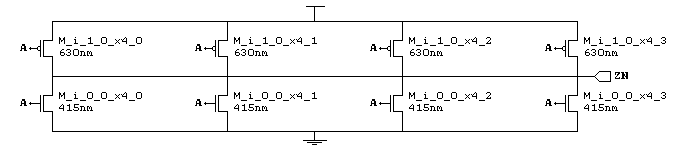
\includegraphics[width=1.2\linewidth]{../INV_X4/INV_X4.png}
	\caption{Reference schematic of the inverter}
	\label{fig:inv_png}
\end{figure}
\begin{figure}[hbtp]
	\centering
	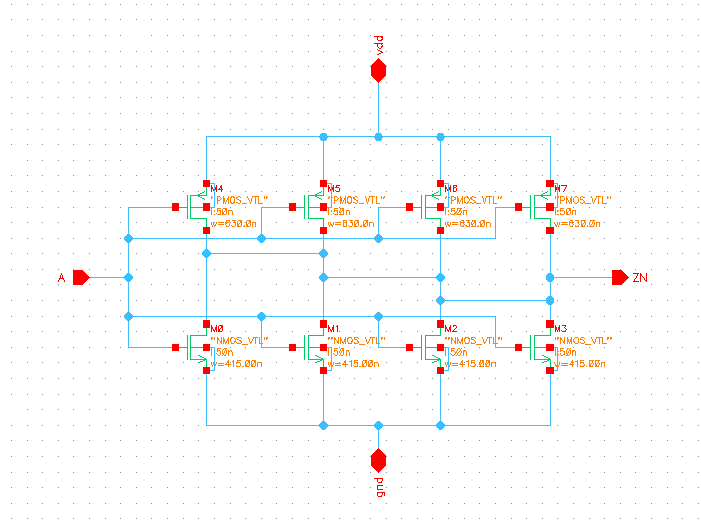
\includegraphics[width=\linewidth]{../INV_X4/INV_X4_schematic.png}
	\caption{Final schematic of \inv}
	\label{fig:inv_schematic}
\end{figure}

We then carried out some preliminary simulations using a test bench, to confirm that the circuit works correctly. We measured rise and fall times, as well as propagation delays, that will be compared with the actual characterization later on. We also measured the transfer characteristic, shown in figure \ref{fig:inv_tchar}.
\begin{figure}[hbtp]
	\centering
	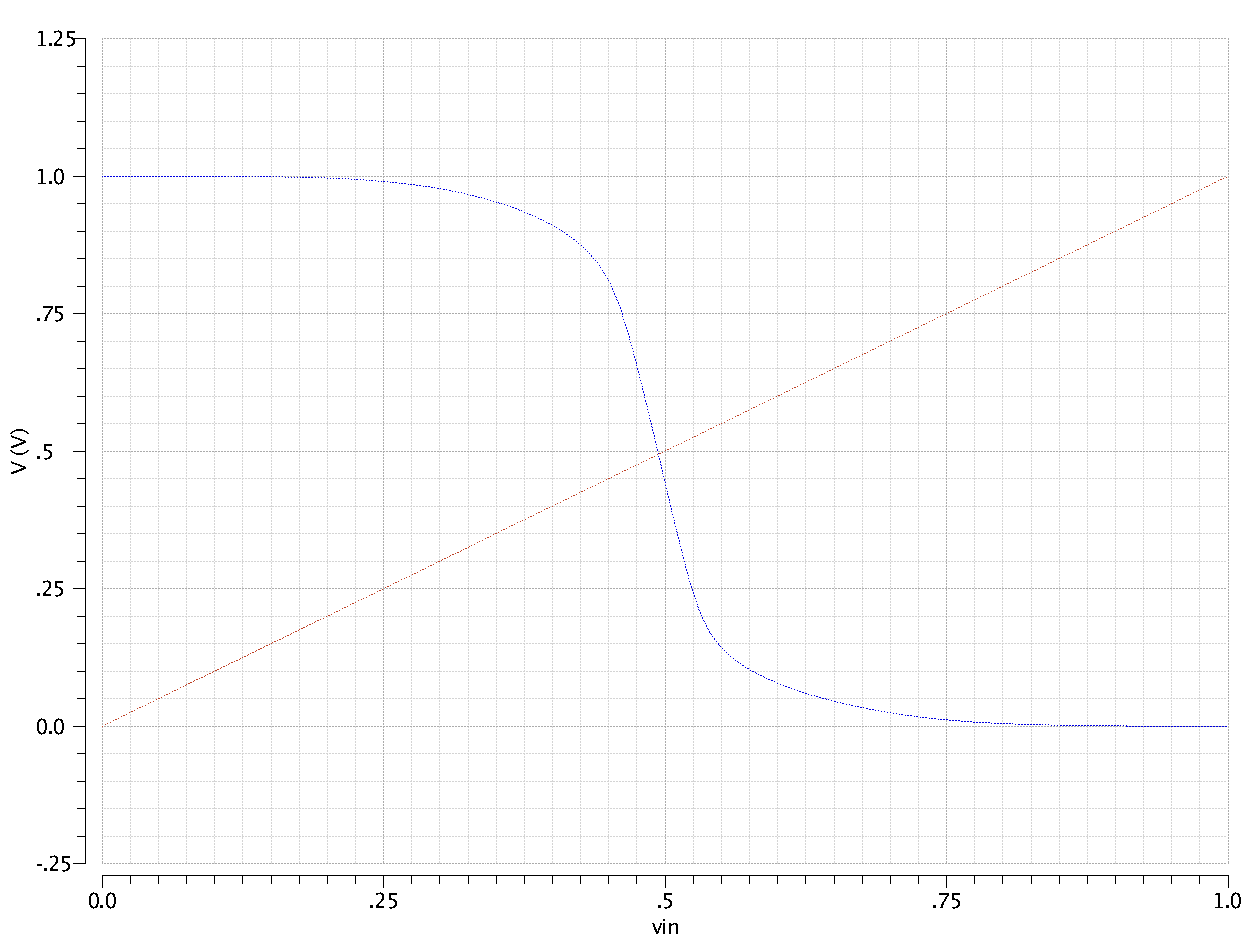
\includegraphics[width=.7\linewidth]{../INV_X4/INV_X4_transfer_char.pdf}
	\caption{Inverter transfer characteristic}
	\label{fig:inv_tchar}
\end{figure}


\subsection{Layout}
\subsection{Characterization}

\section{Half adder}
\subsection{Schematic}
The schematic was drawn using Virtuoso schematic editor.

\subsection{Layout}
Given that the layout of the half adder is quite more complex than the one of the inverter, we started by deeply analyzing the possible approaches using the pen-and-paper method. The final solution that we found consisted in sharing source/drain diffusions as much as possible, in order to minimize the area in the horizontal direction.

When actually drawing the design in Virtuoso, we made sure of running the Design Rule Checker very often, in order to avoid problems in advance.

The design started with the schematic. We tried to put the two outputs on the opposite sides of the cell, because this way the paths input-output are long $\frac{w}{2}$ at maximum, if the inputs are linked
Il design è stato inizialmente fatto carta e penna, guardando lo schematico disegnato. Si è partiti dall'imporre che i due output fossero ai lati estremi della cella, per fare in modo che i percorsi input-output fossero al massimo circa metà della dimensione orizzontale della cella. Tutto questo perché l'intenzione iniziale era quella di mettere i vias per gli input circa a metà cella.

Si è quindi partiti dall'uscita CO per iniziare a disegnare il layout. Abbiamo disegnato il primo nMos dell'inverter e, nell'ottica di condividere il più possibile i sources, abbiamo piazzato il secondo


\subsection{Characterization}

\end{document}
